%%%%%%%%%%%%%%%%%%%%%%%%%%%%%%%%%%%%%%%%%%%%%%%%%%%%%%%%%%%%%%%%%%%%%%
%%                     Modulation
%%%%%%%%%%%%%%%%%%%%%%%%%%%%%%%%%%%%%%%%%%%%%%%%%%%%%%%%%%%%%%%%%%%%%%
%\color{blue}
\subsection{Glyph: \glyph{Modulation}}\label{sec:modulation}

A modulation affects the flux of a process
represented by the target transition. Such a modulation can affect the
process \textbf{positively or negatively}, or even both ways depending on the
conditions, for instance the concentration of the intervening
participants. A \glyph{modulation} can also be used when one does not know the precise direction of the effect.

\begin{glyphDescription}
 \item[SBO]\mbox{}\\ SBO:0000168 ! control
 \item[origin]\mbox{}\\ Any EPN (section~\ref{sec:EPNs}) or any logical operator (section~\ref{sec:logic}).
 \item[target]\mbox{}\\ Any transition node (section~\ref{sec:PNs}).
 \item[end-points]\mbox{}\\ The target extremity of a \glyph{modulation} carries an empty diamond.
 \end{glyphDescription}

\begin{figure}[H]
  \centering
  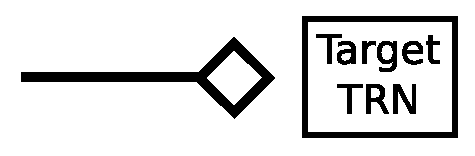
\includegraphics[scale = 0.5]{images/modulation}
  \caption{The \PD glyph for \glyph{modulation}.}
  \label{fig:modulation}
\end{figure}

The following example represents the effect of nicotine on the transition between closed and open states of nicotinic acetylcholine receptor. High concentrations of nicotine open the receptor while low concentrations can desensitize it without opening. 

\begin{center}
\scalebox{0.5}{\includegraphics{examples/modulation-nAChR}}
\end{center}

% The following example represents the effect of the voltage (a unit of information of the membrane compartment) on the opening of a sodium channel voltage-dependent. High depolarisation opens the channels while low depolarisation inactivates it (Note that the same result can be achieved with two irreversible transitions stimulated by two mutually exclusive (using \glyph{and} and \glyph{not}) units of information).
% 
% \begin{center}
% \scalebox{0.5}{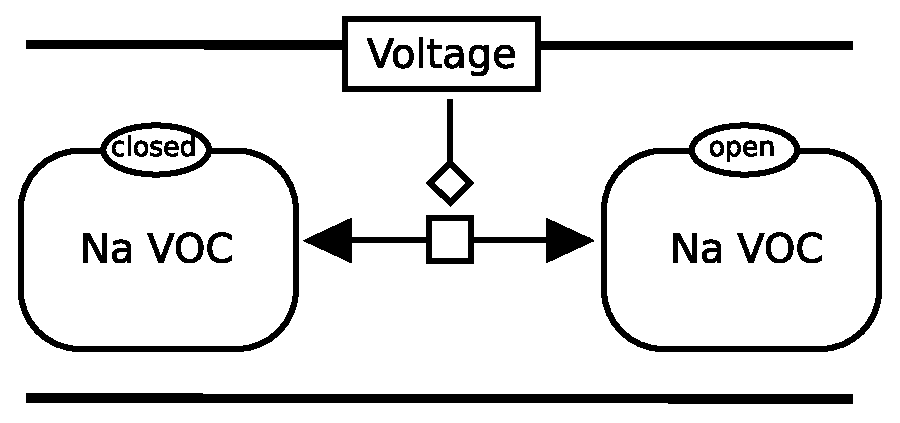
\includegraphics{examples/modulation-VOC}}
% \end{center}

\normalcolor

